% Kompiler med: pdflatex ER-diagram.tex
% For automatisk layout (uten overlapp) trengs LuaLaTeX + graphdrawing; layoutet under er manuelt tilpasset for minimal overlapp.
\documentclass[border=10pt]{standalone}
\usepackage{tikz}
\usepackage{xcolor}
\usepackage{ulem}
\usetikzlibrary{shapes.geometric, shapes.multipart, positioning}

\definecolor{entityblue}{RGB}{173, 216, 230} % light blue

\begin{document}
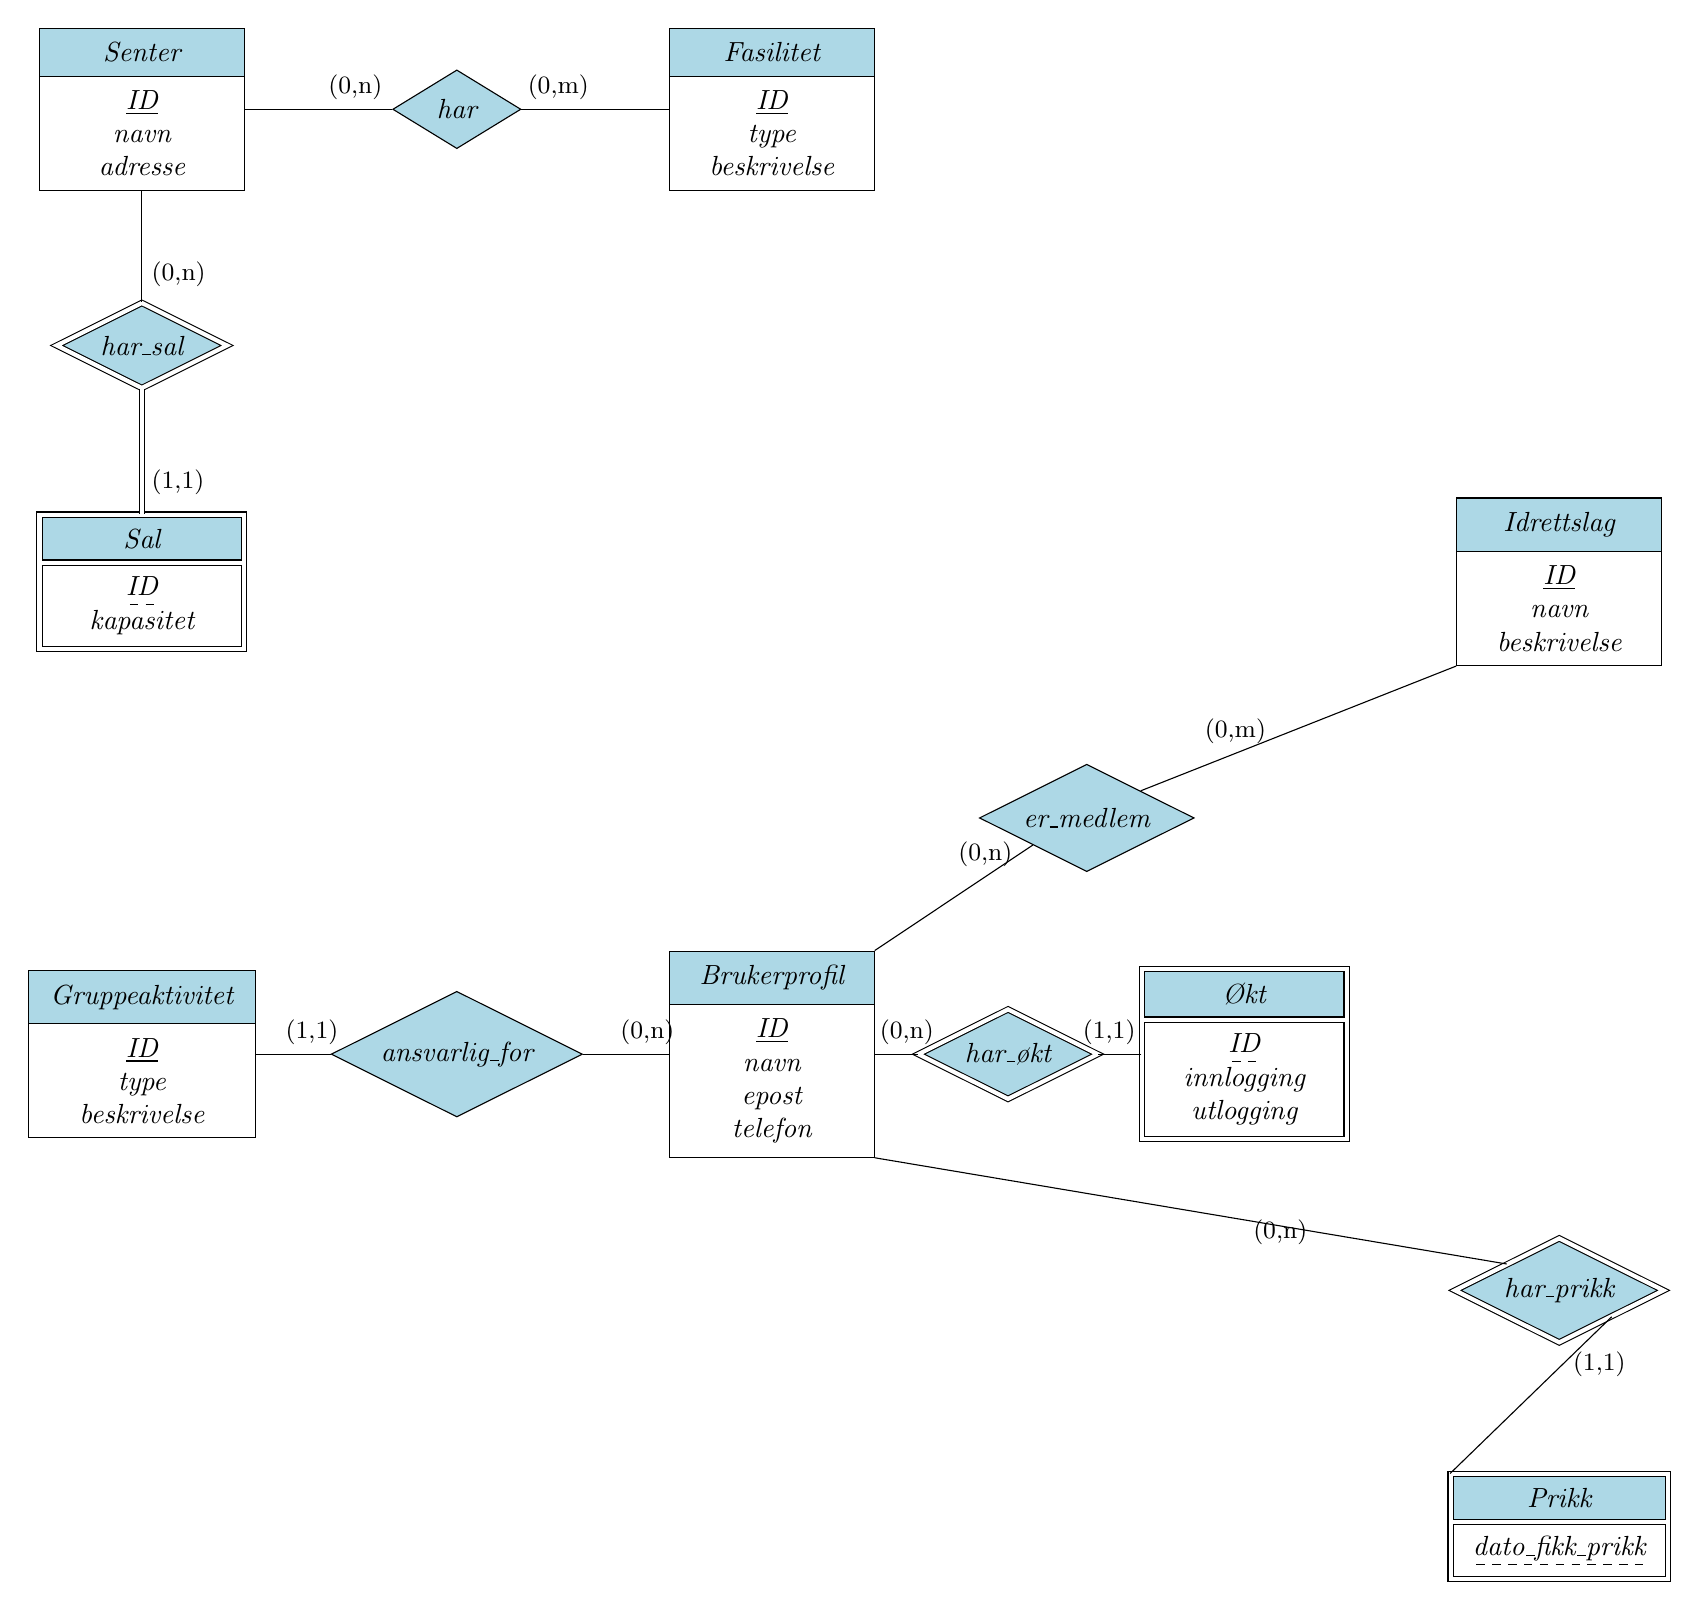
\begin{tikzpicture}[
  font=\itshape,
  entity/.style={
    draw=black,
    rectangle split,
    rectangle split parts=2,
    rectangle split part fill={entityblue, white},
    rectangle split horizontal=false,
    minimum width=2.6cm,
    minimum height=2cm,
    align=center,
    inner xsep=8pt,
    inner ysep=5pt,
    font=\itshape,
  },
  entity part 1/.style={align=center},
  entity part 2/.style={align=left},
  relationship/.style={
    draw=black,
    fill=entityblue,
    diamond,
    aspect=2,
    minimum width=1.5cm,
    minimum height=1cm,
    align=center,
    inner sep=3pt,
  },
  weakentity/.style={
    draw=black,
    double,
    double distance=1.5pt,
    rectangle split,
    rectangle split parts=2,
    rectangle split part fill={entityblue, white},
    rectangle split horizontal=false,
    minimum width=2.6cm,
    minimum height=2cm,
    align=center,
    inner xsep=8pt,
    inner ysep=5pt,
    font=\itshape,
  },
  identifyingrelationship/.style={
    draw=black,
    double,
    double distance=1.5pt,
    fill=entityblue,
    diamond,
    aspect=2,
    minimum width=1.5cm,
    minimum height=1cm,
    align=center,
    inner sep=3pt,
  }
]

  % === VENSTRE KOLONNE (x=0): Senter-stammen + Gruppeaktivitet lenger nede ===
  % Senter-stammen: Senter øverst, deretter har_sal og Sal under
  \node[entity] (senter) at (0, 10) {\normalsize Senter \nodepart{second} \underline{ID}\\ navn\\ adresse};
  \node[identifyingrelationship] (senter-sal) at (0, 7) {\normalsize har\_sal};
  \node[weakentity] (sal) at (0, 4) {\normalsize Sal \nodepart{second} \dashuline{ID}\\ kapasitet};
  % Gruppeaktivitet tydelig under Sal (stor vertikal avstand)
  \node[entity] (gruppe) at (0, -2) {\normalsize Gruppeaktivitet \nodepart{second} \underline{ID}\\ type \\ beskrivelse};

  % === ØVERSTE RAD (y=10): Senter -- har -- Fasilitet ===
  \node[relationship] (senter-fasilitet) at (4, 10) {\normalsize har};
  \node[entity] (fasilitet) at (8, 10) {\normalsize Fasilitet \nodepart{second} \underline{ID}\\ type \\ beskrivelse};

  % === MIDTRAD (y=-2): Gruppeaktivitet -- ansvarlig_for -- Brukerprofil -- har_økt -- Økt ===
  \node[relationship] (ansvarlig-for) at (4, -2) {\normalsize ansvarlig\_for};
  \node[entity] (bruker) at (8, -2) {\normalsize Brukerprofil \nodepart{second} \underline{ID}\\ navn\\ epost \\ telefon};
  \node[identifyingrelationship] (bruker-okt) at (11, -2) {\normalsize har\_økt};
  \node[weakentity] (okt) at (14, -2) {\normalsize Økt \nodepart{second} \dashuline{ID}\\ innlogging \\ utlogging};

  % === HØYRE KOLONNE (x=18): Idrettslag, har_prikk, Prikk ===
  \node[relationship] (er-medlem) at (12, 1) {\normalsize er\_medlem};
  \node[entity] (idrett) at (18, 4) {\normalsize Idrettslag \nodepart{second} \underline{ID}\\ navn\\ beskrivelse};
  \node[identifyingrelationship] (bruker-prikk) at (18, -5) {\normalsize har\_prikk};
  \node[weakentity] (prikk) at (18, -8) {\normalsize Prikk \nodepart{second} \dashuline{dato\_fikk\_prikk}};

  % Kantene med kardinaliteter
  \draw (senter.east) -- (senter-fasilitet.west) node[pos=0.75, above, font=\normalfont\small] {(0,n)};
  \draw (fasilitet.west) -- (senter-fasilitet.east) node[pos=0.75, above, font=\normalfont\small] {(0,m)};
  \draw (senter.south) -- (senter-sal.north) node[pos=0.75, right, font=\normalfont\small] {(0,n)};
  \draw[double, double distance=1.5pt] (senter-sal.south) -- (sal.north) node[pos=0.75, right, font=\normalfont\small] {(1,1)};
  \draw (gruppe.east) -- (ansvarlig-for.west) node[pos=0.75, above, font=\normalfont\small] {(1,1)};
  \draw (ansvarlig-for.east) -- (bruker.west) node[pos=0.75, above, font=\normalfont\small] {(0,n)};
  \draw (bruker.east) -- (bruker-okt.west) node[pos=0.75, above, font=\normalfont\small] {(0,n)};
  \draw (okt.west) -- (bruker-okt.east) node[pos=0.75, above, font=\normalfont\small] {(1,1)};
  \draw (bruker.south east) -- (bruker-prikk.north west) node[pos=0.7, left, font=\normalfont\small] {(0,n)};
  \draw (prikk.north west) -- (bruker-prikk.south east) node[pos=0.7, right, font=\normalfont\small] {(1,1)};
  \draw (bruker.north east) -- (er-medlem.south west) node[pos=0.7, above, font=\normalfont\small] {(0,n)};
  \draw (idrett.south west) -- (er-medlem.north east) node[pos=0.7, above, font=\normalfont\small] {(0,m)};

\end{tikzpicture}

\vspace{1.5cm}

\begin{tikzpicture}[
  font=\itshape,
  entityheader/.style={
    draw=black,
    fill=entityblue,
    minimum width=2cm,
    minimum height=0.5cm,
    align=center,
  },
  entitybody/.style={
    draw=black,
    fill=white,
    minimum width=2cm,
    minimum height=1cm,
    align=left,
    inner xsep=6pt,
    inner ysep=4pt,
  },
  relationship/.style={
    draw=black,
    fill=entityblue,
    diamond,
    aspect=2,
    minimum width=1.4cm,
    minimum height=0.9cm,
    align=center,
    inner sep=2pt,
  }
]
\end{tikzpicture}
\end{document}

